%!TEX root = ../thesis.tex
\documentclass[12pt]{article}

\RequirePackage{graphicx}

\title{Mosaic alignments for paper `Gene conversion drives allelic dimorphism in two
paralogous surface antigens of the malaria parasite \textit{P. falciparum}'}
\date{February 2023}

\begin{document}
\maketitle

\graphicspath{{img/}}


\clearpage

\begin{figure}
    \centering
    \centerline{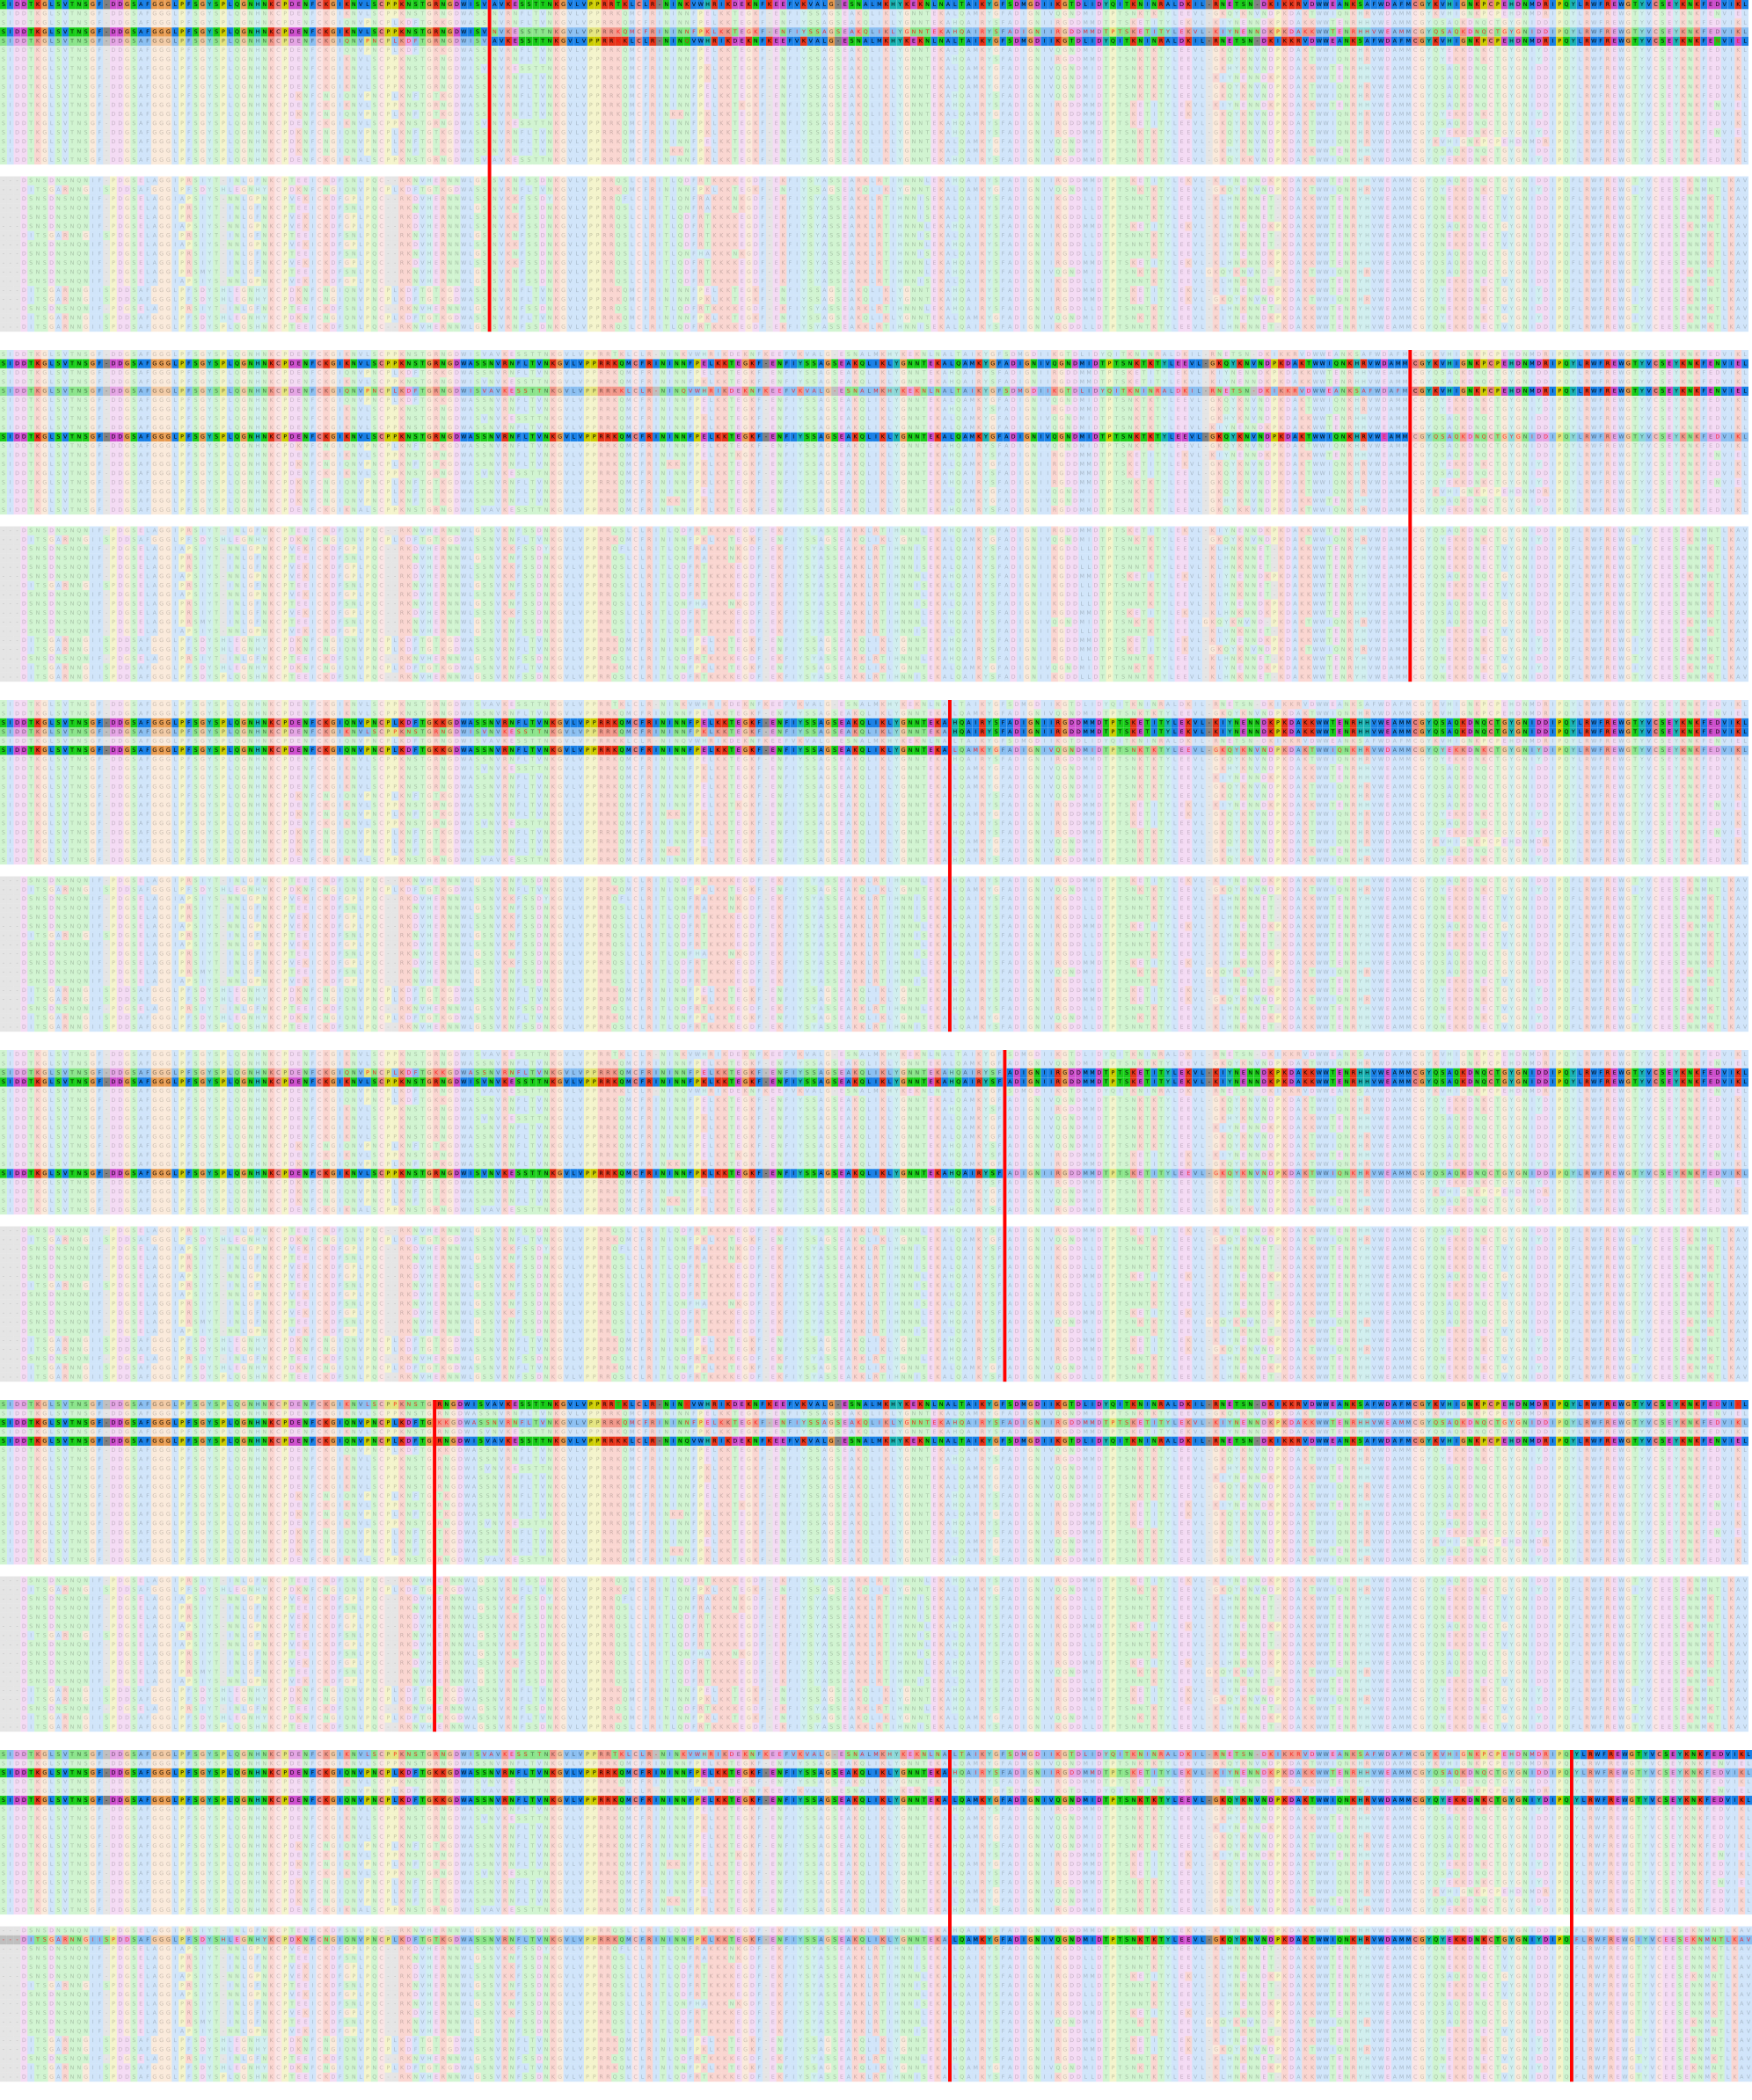
\includegraphics[width=1.2\textwidth]{DBLMSP_ref_FP0009-C_FP0030-C_FP0068-C_FP0081-C_PA0074-C.png}}
    \caption[Mosaic alignments (1)]{
        \textbf{Mosaic alignments for gene DBLMSP in samples 3D7, FP0009-C, FP0030-C,
        FP0068-C, FP0081-C, PA0074-C.}
        }
    \label{pa:fig:mosaic_app1}
\end{figure}

\begin{figure}
    \centering
    \centerline{
\includegraphics[width=1.2\textwidth]{DBLMSP_PA0232-C_PC0009-C_PD0075-C_PD0791-C_PD0822-C_PE0089-C.png}}
    \caption[Mosaic alignments (2)]{
        \textbf{Mosaic alignments for gene DBLMSP in samples PA0232-C, PC0009-C,
        PD0075-C, PD0791-C, PD0822-C, PE0089-C.}
        }
    \label{pa:fig:mosaic_app2}
\end{figure}

\begin{figure}
    \centering
    \centerline{
\includegraphics[width=1.2\textwidth]{DBLMSP_PF0098-C_PF0232-C_PF0482-C_PT0007-CW_QP0195-C_QT0006-C.png}}
    \caption[Mosaic alignments (3)]{
        \textbf{Mosaic alignments for gene DBLMSP in samples PF0098-C,
        PF0232-C, PF0482-C, PT0007-CW, QP0195-C, QT0006-C.}
        }
    \label{pa:fig:mosaic_app3}
\end{figure}


\begin{figure}
    \centering
    \centerline{
\includegraphics[width=1.2\textwidth]{DBLMSP2_ref_FP0018-C_FP0021-C_FP0028-C_FP0033-C_FP0062-C.png}}
    \caption[Mosaic alignments (5)]{
        \textbf{Mosaic alignments for gene DBLMSP2 in samples 3D7, FP0018-C, FP0021-C,
        FP0028-C, FP0033-C, FP0062-C.}
        }
    \label{pa:fig:mosaic_app5}
\end{figure}

\begin{figure}
    \centering
    \centerline{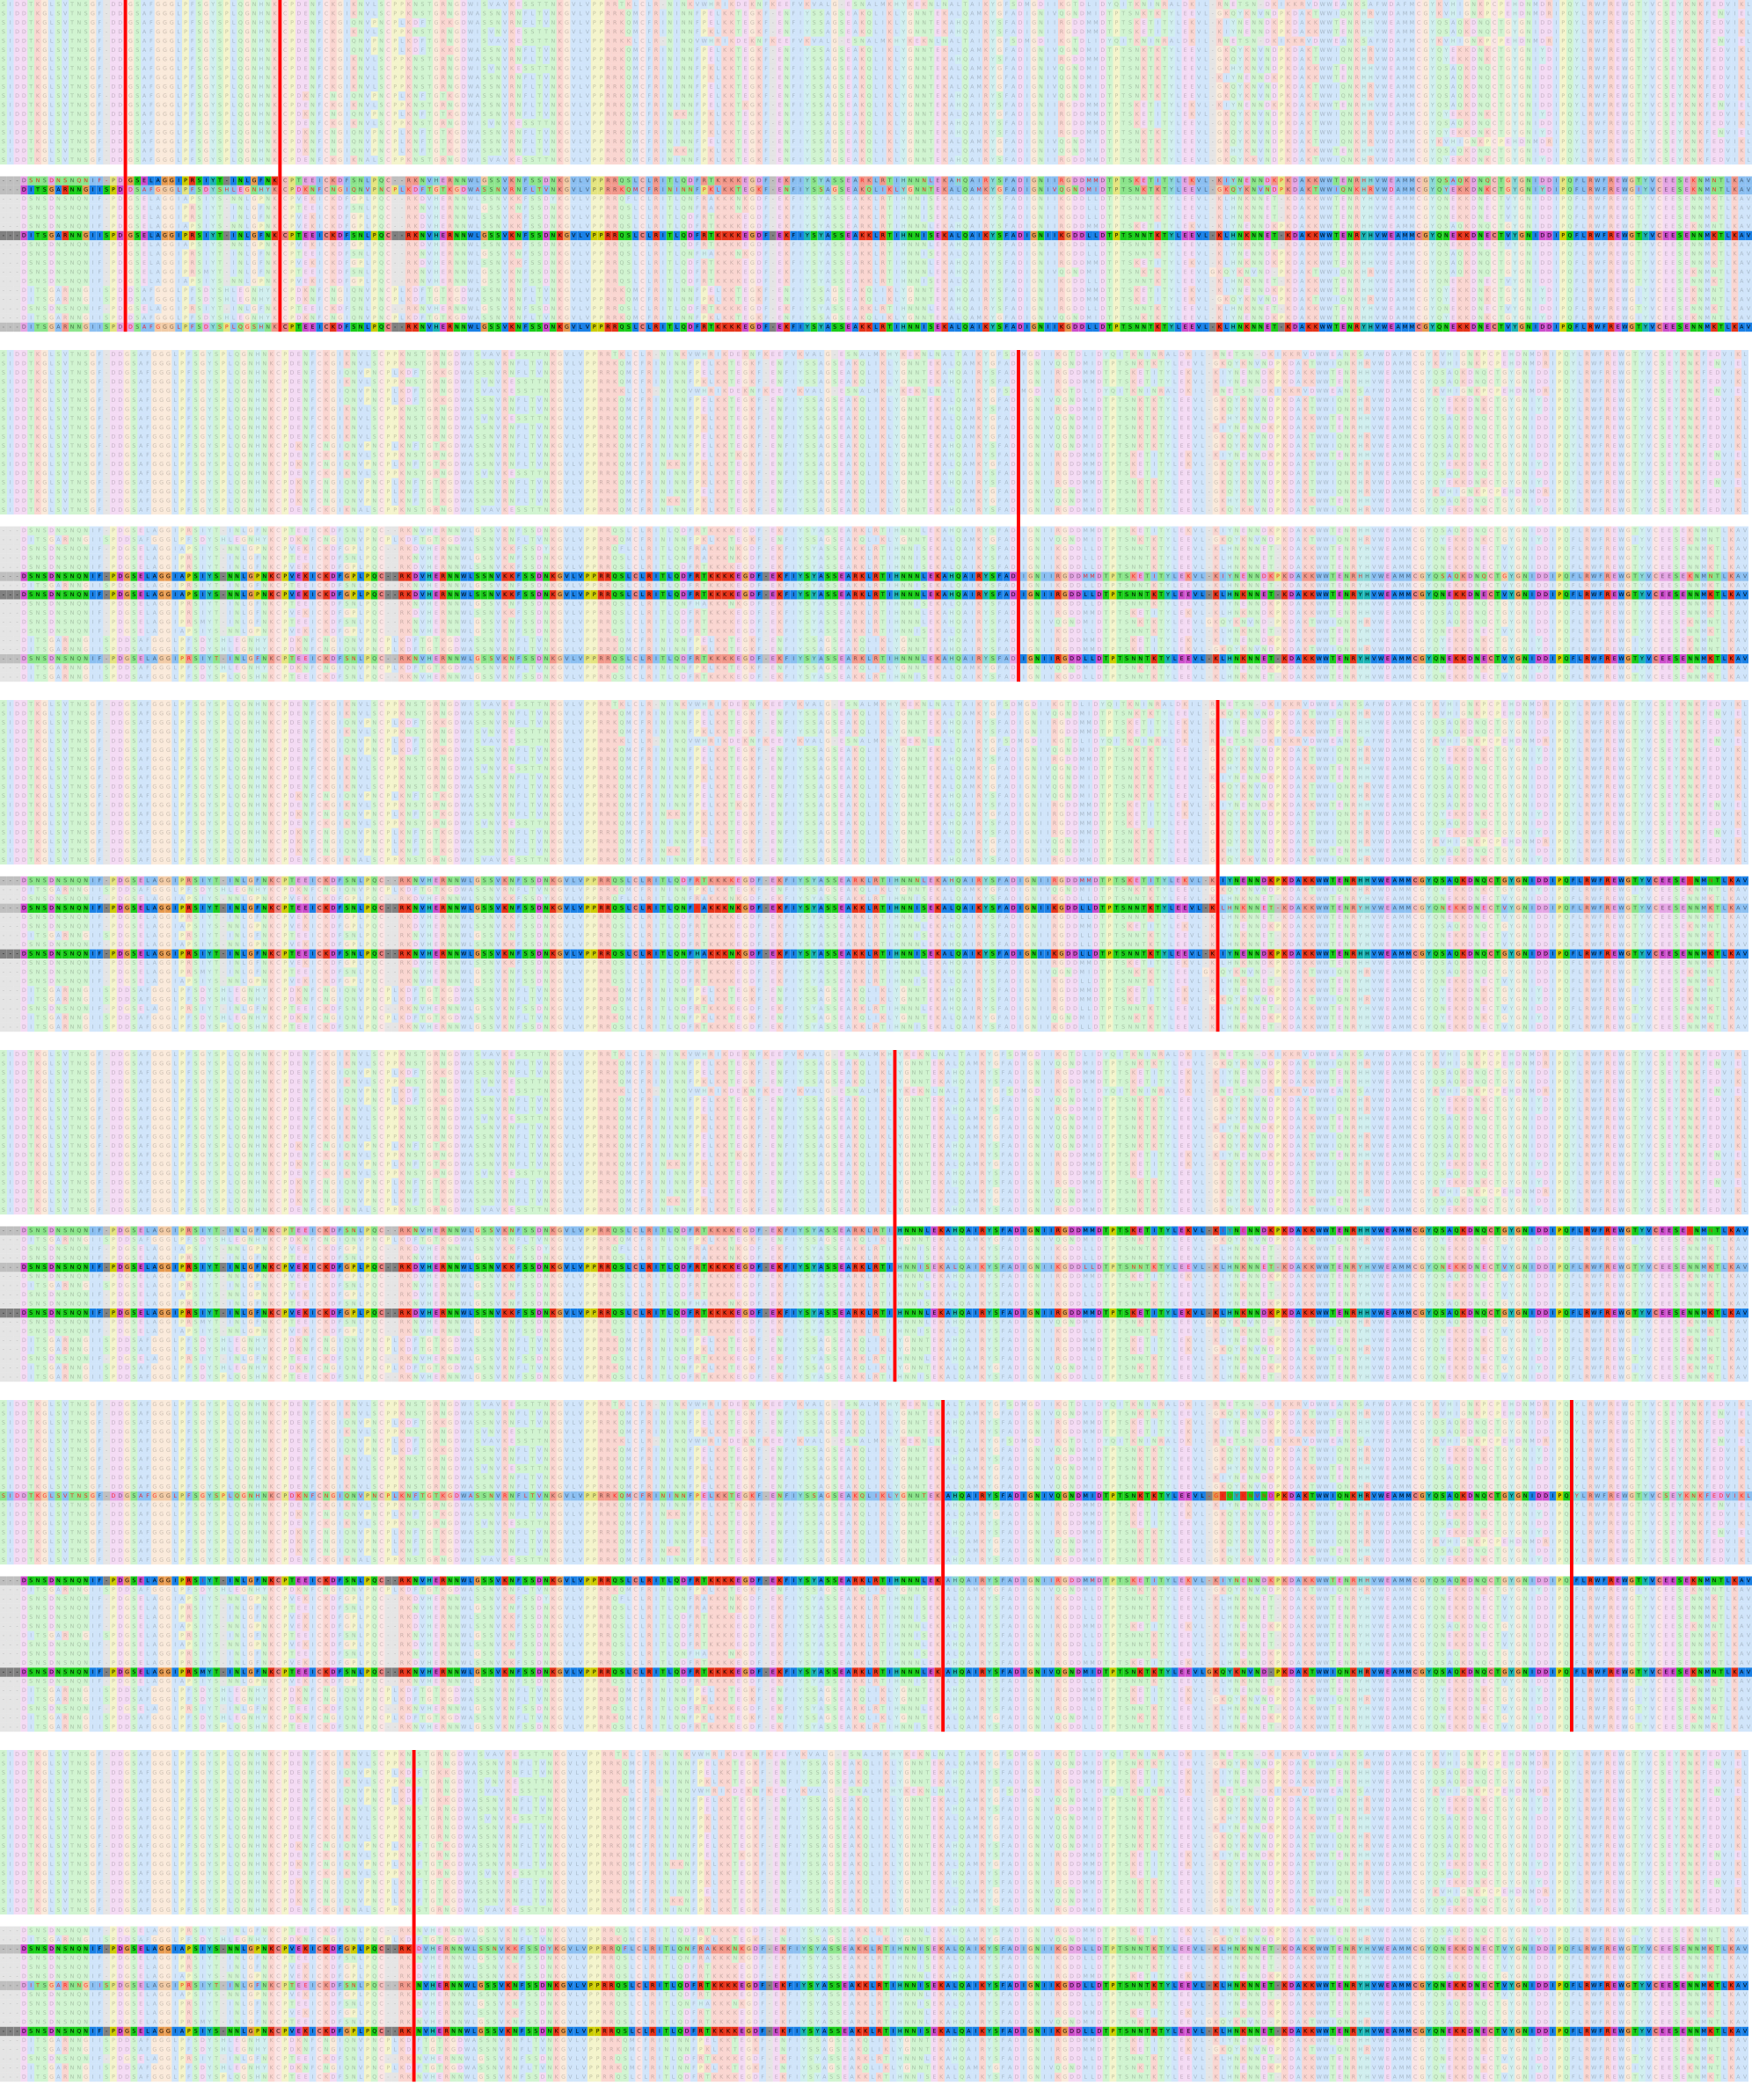
\includegraphics[width=1.2\textwidth]{DBLMSP2_PA0223-C_PA0254-C_PA0419-C_PC0019-C_PC0197-C_PD0461-C.png}}
    \caption[Mosaic alignments (6)]{
        \textbf{Mosaic alignments for gene DBLMSP2 in samples PA0223-C, PA0254-C,
        PA0419-C, PC0019-C, PC0197-C, PD0461-C.}
        }
    \label{pa:fig:mosaic_app6}
\end{figure}

\begin{figure}
    \centering
    \centerline{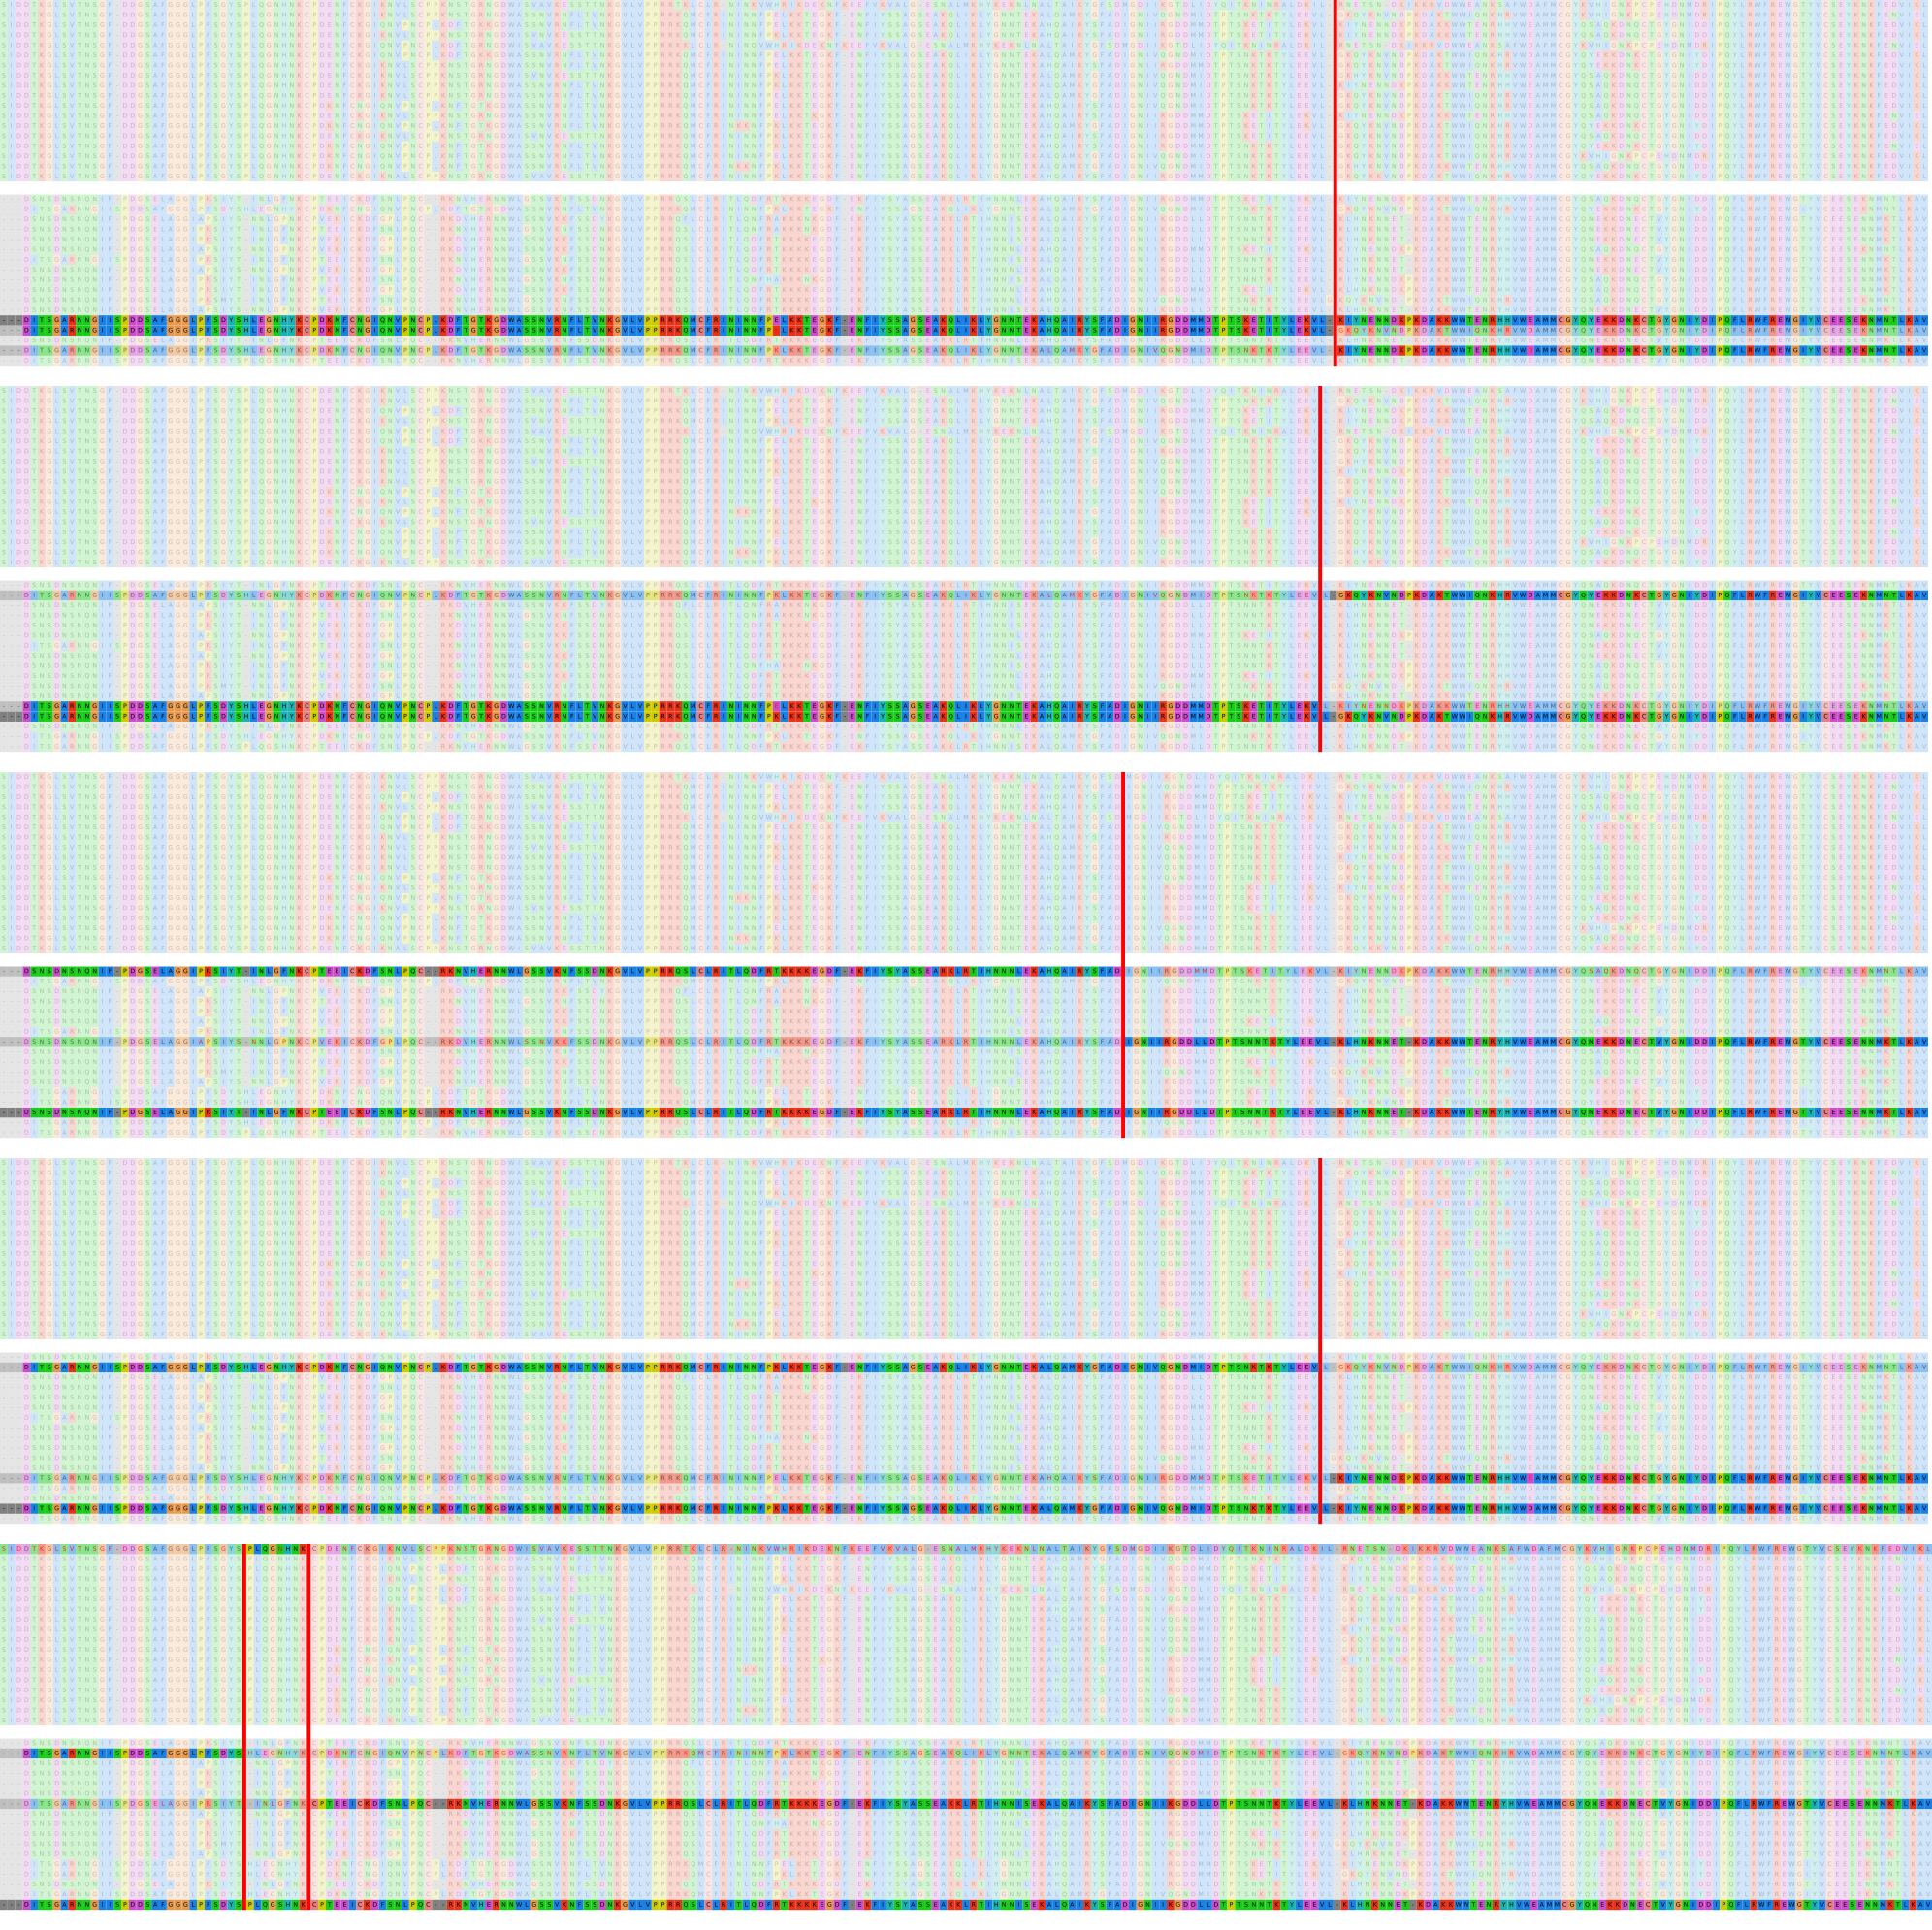
\includegraphics[width=1.2\textwidth]{DBLMSP2_PD0986-C_PD1082-C_PN0020-C_QE0398-C_QQ0063-C.png}}
    \caption[Mosaic alignments (7)]{
        \textbf{Mosaic alignments for gene DBLMSP2 in samples PD0986-C, PD1082-C,
        PN0020-C, QE0398-C, QQ0063-C.}
        }
    \label{pa:fig:mosaic_app7}
\end{figure}


\end{document}
